High energy leptons inside a strong magnetic filed can emit high energy photons.
This is the case for the electrons and muons from the decay of the \PZ and \PW bosons.
The Final State Radiation (FSR) photons emitted by leptons are not included at all in the Particle Flow reconstruction of muon momentum,
and may be missed in electron reconstruction, leading to a degradation of the accuracy for the Z bosons momentum and mass.

In order to improve the reconstruction of the momentum of the leptons, it is necessary to identify FSR photons and associate them to the parent lepton.
This is also important in order to suppress the background from diboson ($\PZ\PZ$ for the 4\Pl channel $\PW\PZ$ for the 3\Pl channel respectively),
where the additional photon does not come from the hard scattering, but is instead radiated by one of the leptons.

The FSR recovery algorithm is designed to discriminate FSR photons from the background from \pileup interactions and from Initial State Radiation (ISR).
This is achieved by exploiting the kinematics of FSR photons, which tend to be collinear to the parent lepton and to be isolated from hadronic activity in the event.

The FSR photons are selected for each lepton, starting from the collection of photons produced by the Particle Flow algorithm.
FSR candidates are required to have transverse momentum $p_{T}^{\gamma} > 2 \GeV$ and pseudorapidity $|\eta^{\gamma}| < 2.4$ (inside the tracker acceptance).
A relative isolation is computed as:
\begin{equation}
I^{\PGg} \mathdefined \frac{1}{\pt^\PGg} \left( \sum{\pt^\PGg} + \sum_{i\, \in\, \mathrm{neutral}}{\pt^i} + \sum_{j\, \in\, \mathrm{charged}}{\pt^j} \right)
\end{equation}
where $\sum{\pt^\PGg}$, $\sum_{i\, \in\, \mathrm{neutral}}{\pt^i}$ and $\sum_{j\, \in\, \mathrm{charged}}{\pt^j}$
are the scalar sums of the transverse momenta of photons, neutral and charged hadrons inside a cone of radius $\mathrm{R} = 0.3$ around the photon,
including \pileup contributions.
It is required that the relative isolation is $I^{\PGg} < 1.8$.

The photons that passed these selections are associated to the closest lepton, among those that pass the loose ID and SIP cut (see Section \ref{sec:eleSIP}).
Because the electron reconstruction algorithm already recovers some of the FSR photons, we exclude those that have $\Delta R(e, \gamma) <$ 0.15 or $|\Delta\phi(e, \gamma)| <$ 2 and $|\Delta\eta(e, \gamma)| <$ 0.05 to avoid double counting.
The FSR candidates are also discarded if they do not satisfy $\Delta R(\ell, \gamma) < 0.5$ with respect to the associated lepton.

FSR photons tend to have higher energies than the ones from \pileup or from hadronic decays (e.g. \PGpz\,),
and are expected to be quasi-collinear with the emitting leptons.
The candidate with the smallest $\Delta R(\ell, \gamma)\, / E_{T,\gamma}^{2}$ is kept,
and is accepted only if $\Delta R(\ell, \gamma)\, / E_{T,\gamma}^{2} < 0.012 \GeV^{-2}$.
Accepted FSR photons have their momentum added to the lepton and are excluded from the computation of its isolation.

A detailed study on the optimization of the FSR recovery algorithm can be found in Reference \cite{Sirunyan2017}.

Since our analysis selection requires signal photons to have at least $\Delta R(\ell, \gamma) > 0.5$ from any signal lepton, there is no risk of double counting photons.
However thir kinematic distributions were studied, as well as their shower shape variables.
For example, their \pt and $\eta$ distributions can be seen in Figure~\ref{fig:distributions_fsrPhotons}.

\begin{figure}
  \centering
  \hfill
  \subfigure [Transverse momentum] {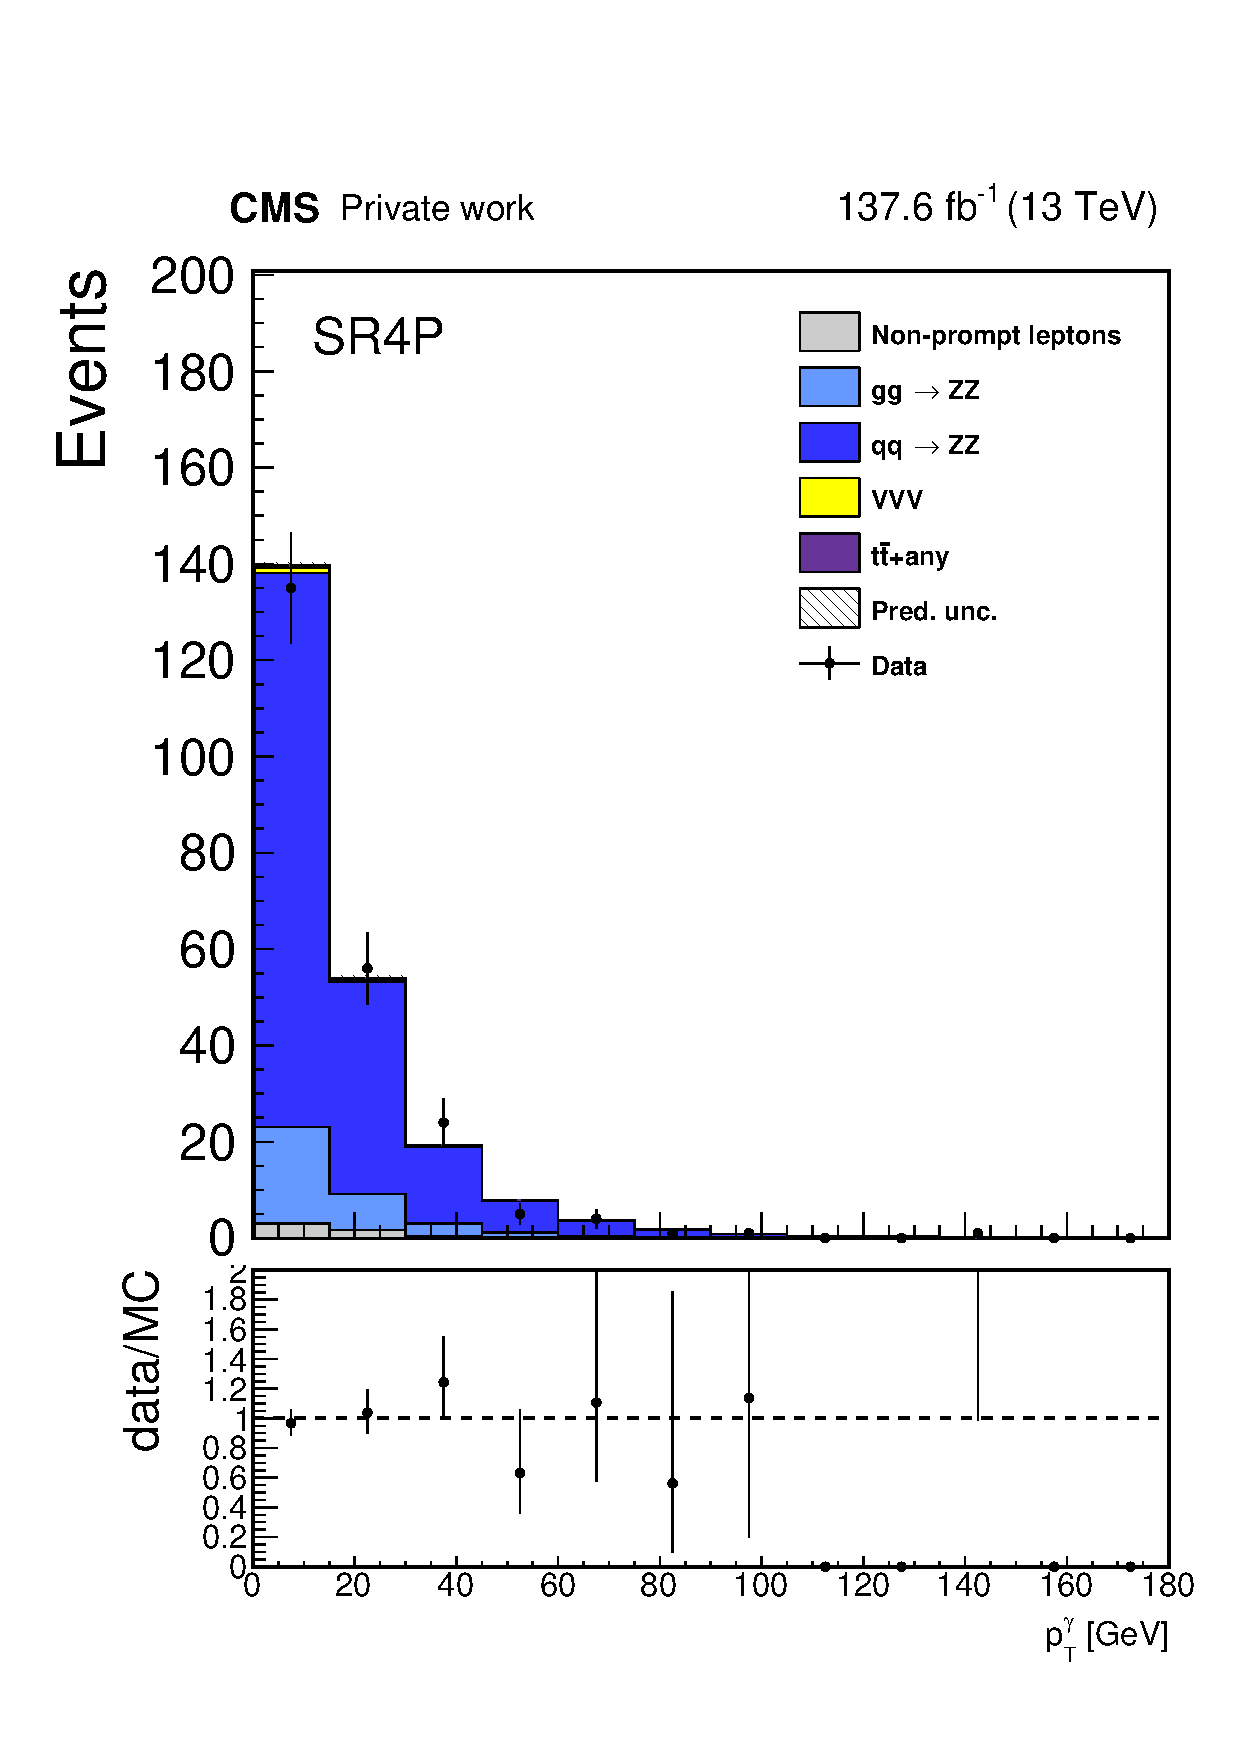
\includegraphics[width=.4\textwidth]{Figures/dataMC/Run2/lepCR/SR4P/lead_fsrPhotons_pt_pow.pdf}}
  \hfill
  \subfigure [Pseudorapidity]      {\includegraphics[width=.4\textwidth]{Figures/dataMC/Run2/lepCR/SR4P/lead_fsrPhotons_eta_pow.pdf}}
  \hfill\mbox{}
  \caption{Transverse momentum and pseudorapidity distributions of FSR photons associated to a lepton in the inclusive region with four charged leptons for \RunII.}
  \label{fig:distributions_fsrPhotons}
\end{figure}

%% \begin{figure}
%% \begin{center}
%%         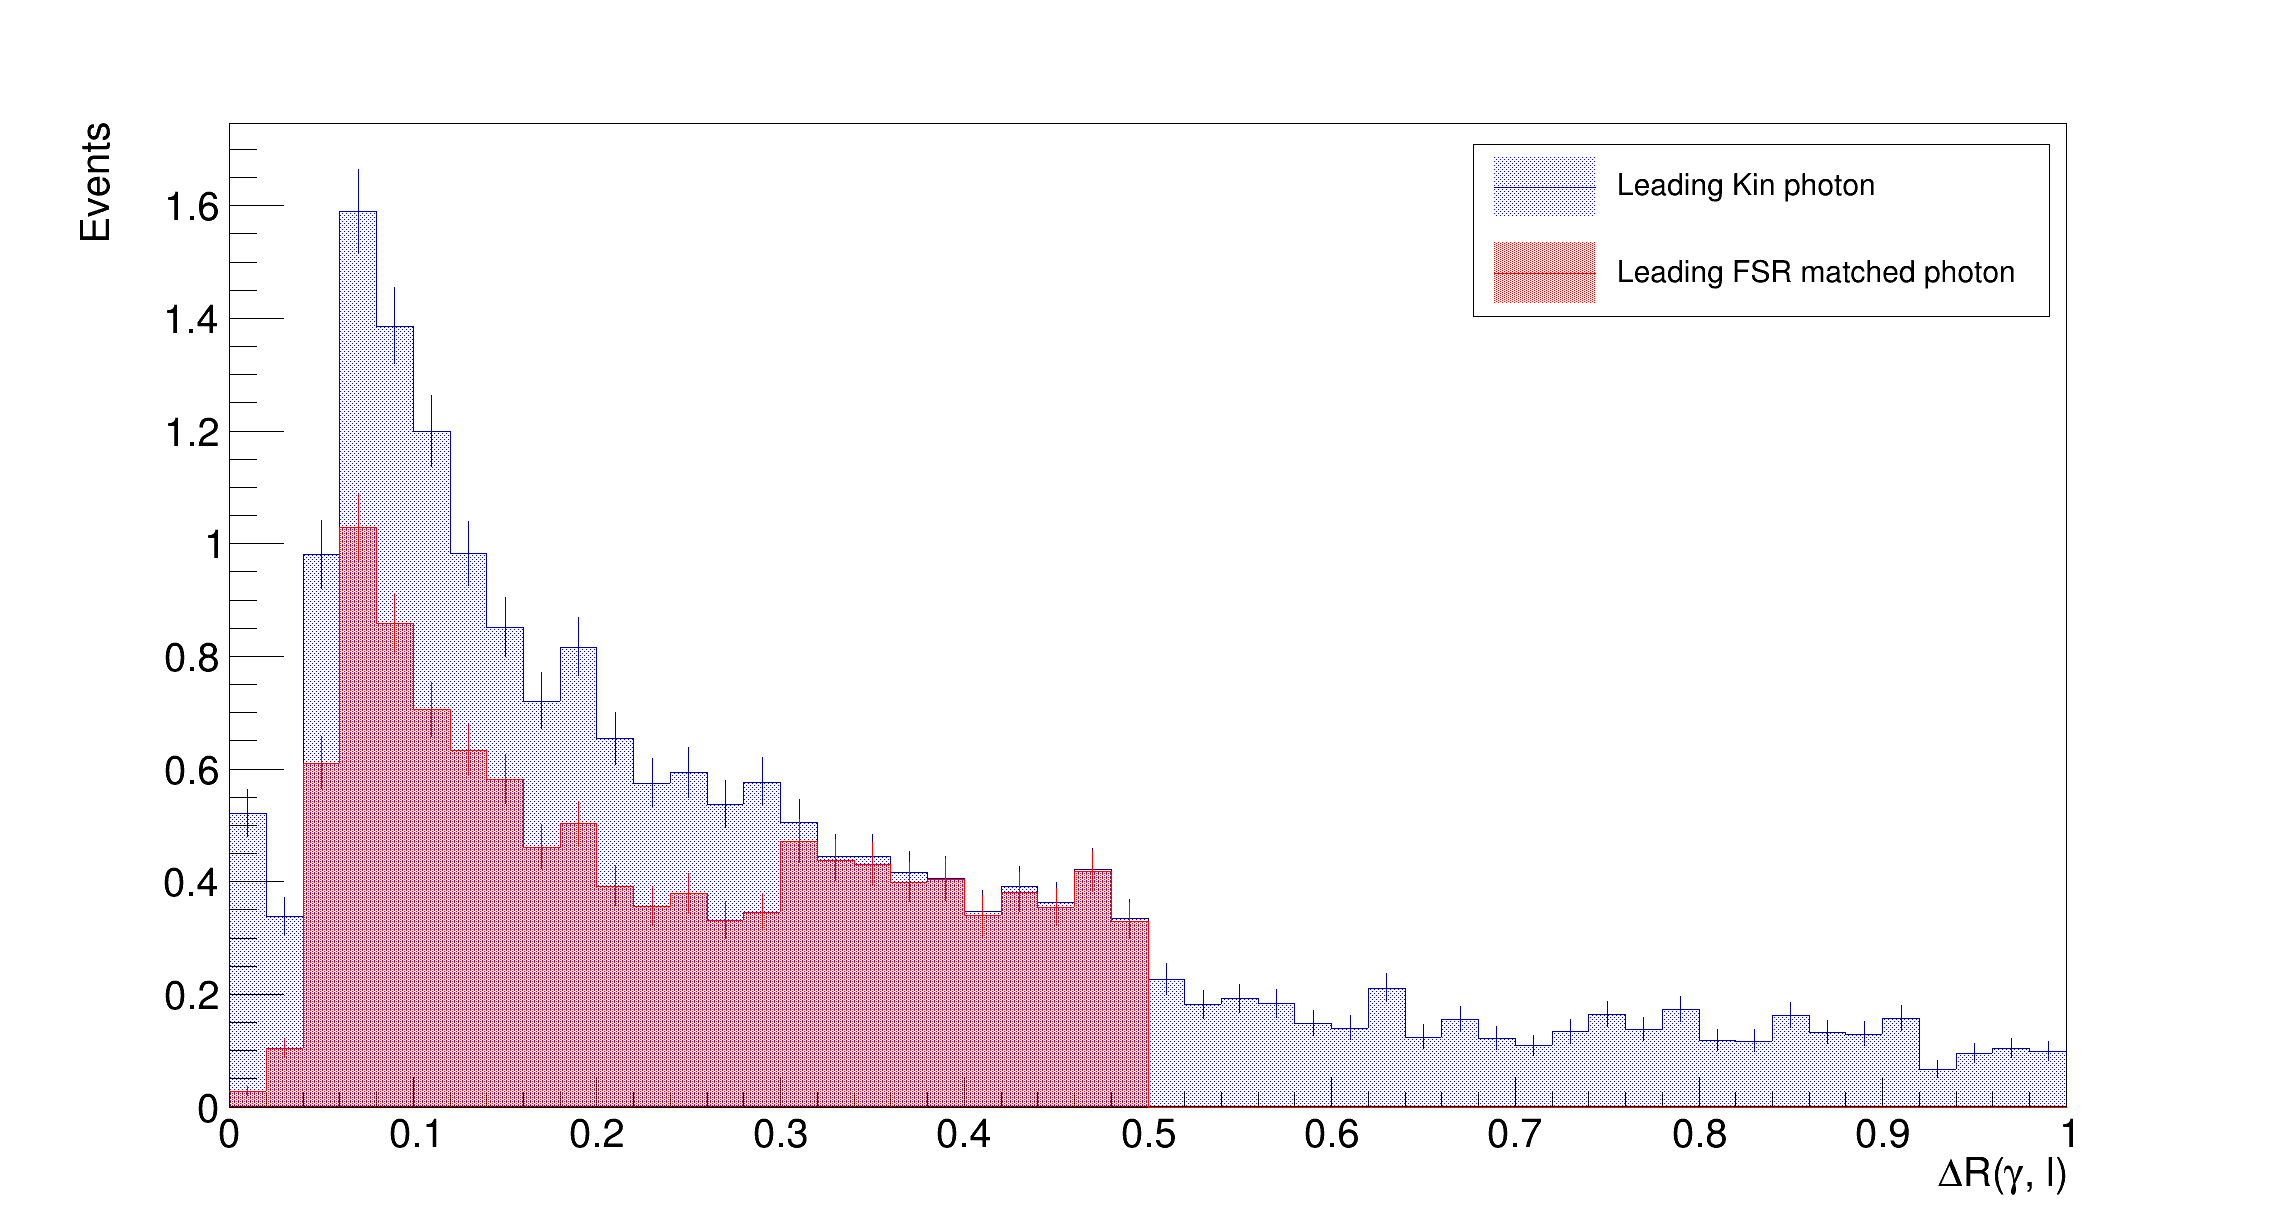
\includegraphics[width=0.8\textwidth]{Figures/lead_dRl_kin_vs_fsrMatched_rebinned.png}
%% \end{center}
%% \caption{$\Delta R(\ell, \gamma)$ for all the photons passing at least the `kinematic' selection with the $\Delta R$ cut relaxed, and for those selected as FSR in the ZZ$\gamma$ sample 2018.}
%% \label{fig:dRl_fsr_photons}
%% \end{figure}

% and the effect of not excluding FSR photons from the computation of the nonprompt rate
